% PARTE 3: EJERCICIOS PROPUESTOS Y SOLUCIONES
% Guía de Identidades Trigonométricas - Grado 10

\section{Ejercicios Propuestos}

Ahora es tu turno de poner en práctica todo lo que has aprendido sobre identidades trigonométricas. ¡Recuerda que las identidades son como herramientas en una caja de herramientas: cada una tiene su momento perfecto para ser usada!

\begin{ejercicio}[title=Ejercicio 1: Identidades Recíprocas]
Usando las identidades recíprocas, simplifica las siguientes expresiones:
\begin{itemize}
    \item[a)] $\sin\theta \cdot \csc\theta + \cos\theta \cdot \sec\theta$
    \item[b)] $\frac{\csc\alpha}{\sec\alpha} \cdot \tan\alpha$
    \item[c)] Si $\sin x = \frac{3}{5}$ y $x$ está en el primer cuadrante, encuentra $\csc x$ y $\cot x$.
\end{itemize}
\end{ejercicio}

\begin{ejercicio}[title=Ejercicio 2: Identidades Pitagóricas]
Aplica las identidades pitagóricas para resolver:
\begin{itemize}
    \item[a)] Si $\cos\theta = \frac{4}{5}$ y $\theta$ está en el cuarto cuadrante, encuentra $\sin\theta$ y $\tan\theta$.
    \item[b)] Simplifica: $1 - \sin^2x + \cos^2x$
    \item[c)] Verifica que $\sec^2\beta - \tan^2\beta = 1$ para $\beta = 30°$
\end{itemize}
\end{ejercicio}

\begin{ejercicio}[title=Ejercicio 3: Simplificación de Expresiones]
Simplifica las siguientes expresiones trigonométricas:
\begin{itemize}
    \item[a)] $\frac{\sin\theta \cos\theta}{\tan\theta}$
    \item[b)] $\frac{1 + \tan^2x}{\sec^2x}$
    \item[c)] $\frac{\sin^2\alpha - \cos^2\alpha}{\sin\alpha - \cos\alpha}$
\end{itemize}
\end{ejercicio}

\begin{ejercicio}[title=Ejercicio 4: Expresar Funciones en Términos de Otras]
\begin{itemize}
    \item[a)] Si $\tan\theta = t$, expresa $\sin\theta$ y $\cos\theta$ en términos de $t$ (considera $\theta$ en el primer cuadrante).
    \item[b)] Si $\sin x = s$, expresa todas las demás funciones trigonométricas en términos de $s$ (considera $x$ en el segundo cuadrante).
\end{itemize}
\end{ejercicio}

\begin{ejercicio}[title=Ejercicio 5: Demostración de Identidades]
Demuestra las siguientes identidades:
\begin{itemize}
    \item[a)] $\frac{1 - \cos\theta}{\sin\theta} = \frac{\sin\theta}{1 + \cos\theta}$
    \item[b)] $\frac{\tan x + \cot x}{\sec x \cdot \csc x} = 1$
\end{itemize}
\end{ejercicio}

\begin{ejercicio}[title=Ejercicio 6: Identidades de Suma y Diferencia]
Usando las identidades de suma y diferencia de ángulos:
\begin{itemize}
    \item[a)] Calcula el valor exacto de $\sin(75°)$ usando $\sin(45° + 30°)$
    \item[b)] Encuentra $\cos(15°)$ usando $\cos(45° - 30°)$
    \item[c)] Si $\sin A = \frac{3}{5}$ y $\cos B = \frac{12}{13}$, donde $A$ y $B$ están en el primer cuadrante, encuentra $\sin(A + B)$.
\end{itemize}
\end{ejercicio}

\begin{ejercicio}[title=Ejercicio 7: Identidades de Ángulo Doble]
Aplica las identidades de ángulo doble:
\begin{itemize}
    \item[a)] Si $\sin\theta = \frac{1}{3}$ y $\theta$ está en el primer cuadrante, encuentra $\sin(2\theta)$ y $\cos(2\theta)$.
    \item[b)] Simplifica: $\frac{\sin(2x)}{2\cos x}$
    \item[c)] Demuestra que $\cos(2\alpha) = 2\cos^2\alpha - 1$
\end{itemize}
\end{ejercicio}

\begin{ejercicio}[title=Ejercicio 8: Identidades de Ángulo Medio]
Resuelve usando identidades de ángulo medio:
\begin{itemize}
    \item[a)] Encuentra el valor exacto de $\sin(22.5°)$ usando la identidad de ángulo medio.
    \item[b)] Si $\cos\theta = \frac{7}{25}$ y $0° < \theta < 90°$, encuentra $\sin\left(\frac{\theta}{2}\right)$ y $\cos\left(\frac{\theta}{2}\right)$.
\end{itemize}
\end{ejercicio}

\begin{ejercicio}[title=Ejercicio 9: Transformaciones Producto-Suma]
Transforma los siguientes productos en sumas o diferencias:
\begin{itemize}
    \item[a)] $2\sin(3x)\cos(2x)$
    \item[b)] $\cos(4\theta)\cos(2\theta)$
    \item[c)] $\sin(5\alpha)\sin(3\alpha)$
\end{itemize}
\end{ejercicio}

\begin{ejercicio}[title=Ejercicio 10: Transformaciones Suma-Producto]
Convierte las siguientes sumas o diferencias en productos:
\begin{itemize}
    \item[a)] $\sin(7x) + \sin(3x)$
    \item[b)] $\cos(5\beta) - \cos(3\beta)$
    \item[c)] $\sin(4\theta) - \sin(2\theta)$
\end{itemize}
\end{ejercicio}

\newpage

\section{Soluciones Detalladas}

¡Vamos a resolver cada ejercicio paso a paso! Recuerda que en trigonometría, hay muchos caminos para llegar a la misma respuesta. Lo importante es que cada paso esté bien justificado.

\begin{solucion}[title=Solución Ejercicio 1: Identidades Recíprocas]

\textbf{Parte a):} Simplificar $\sin\theta \cdot \csc\theta + \cos\theta \cdot \sec\theta$

Recordemos las identidades recíprocas:
- $\csc\theta = \frac{1}{\sin\theta}$, entonces $\sin\theta \cdot \csc\theta = 1$
- $\sec\theta = \frac{1}{\cos\theta}$, entonces $\cos\theta \cdot \sec\theta = 1$

Por lo tanto:
\begin{align*}
\sin\theta \cdot \csc\theta + \cos\theta \cdot \sec\theta &= \sin\theta \cdot \frac{1}{\sin\theta} + \cos\theta \cdot \frac{1}{\cos\theta} \\
&= 1 + 1 \\
&= 2
\end{align*}

\textbf{Respuesta:} $\boxed{2}$

\textbf{Parte b):} Simplificar $\frac{\csc\alpha}{\sec\alpha} \cdot \tan\alpha$

Primero expresamos todo en términos de seno y coseno:
\begin{align*}
\frac{\csc\alpha}{\sec\alpha} \cdot \tan\alpha &= \frac{1/\sin\alpha}{1/\cos\alpha} \cdot \frac{\sin\alpha}{\cos\alpha} \\
&= \frac{1}{\sin\alpha} \cdot \frac{\cos\alpha}{1} \cdot \frac{\sin\alpha}{\cos\alpha} \\
&= \frac{\cos\alpha}{\sin\alpha} \cdot \frac{\sin\alpha}{\cos\alpha} \\
&= 1
\end{align*}

\textbf{Respuesta:} $\boxed{1}$

\textbf{Parte c):} Si $\sin x = \frac{3}{5}$ y $x$ está en el primer cuadrante, encontrar $\csc x$ y $\cot x$.

Paso 1: Encontrar $\csc x$ (es la recíproca del seno)
\[
\csc x = \frac{1}{\sin x} = \frac{1}{3/5} = \frac{5}{3}
\]

Paso 2: Para encontrar $\cot x$, primero necesitamos $\cos x$.
Usando la identidad pitagórica $\sin^2x + \cos^2x = 1$:
\begin{align*}
\left(\frac{3}{5}\right)^2 + \cos^2x &= 1 \\
\frac{9}{25} + \cos^2x &= 1 \\
\cos^2x &= 1 - \frac{9}{25} = \frac{16}{25} \\
\cos x &= \frac{4}{5} \quad \text{(positivo porque estamos en el primer cuadrante)}
\end{align*}

Paso 3: Calcular $\cot x$
\[
\cot x = \frac{\cos x}{\sin x} = \frac{4/5}{3/5} = \frac{4}{3}
\]

\textbf{Respuesta:} $\boxed{\csc x = \frac{5}{3}, \quad \cot x = \frac{4}{3}}$
\end{solucion}

\begin{solucion}[title=Solución Ejercicio 2: Identidades Pitagóricas]

\textbf{Parte a):} Si $\cos\theta = \frac{4}{5}$ y $\theta$ está en el cuarto cuadrante, encontrar $\sin\theta$ y $\tan\theta$.

Paso 1: Usar la identidad pitagórica fundamental $\sin^2\theta + \cos^2\theta = 1$
\begin{align*}
\sin^2\theta + \left(\frac{4}{5}\right)^2 &= 1 \\
\sin^2\theta + \frac{16}{25} &= 1 \\
\sin^2\theta &= 1 - \frac{16}{25} = \frac{9}{25} \\
\sin\theta &= \pm\frac{3}{5}
\end{align*}

Como $\theta$ está en el cuarto cuadrante, $\sin\theta < 0$, entonces:
\[
\sin\theta = -\frac{3}{5}
\]

Paso 2: Calcular $\tan\theta$
\[
\tan\theta = \frac{\sin\theta}{\cos\theta} = \frac{-3/5}{4/5} = -\frac{3}{4}
\]

\textbf{Respuesta:} $\boxed{\sin\theta = -\frac{3}{5}, \quad \tan\theta = -\frac{3}{4}}$

\textbf{Parte b):} Simplificar $1 - \sin^2x + \cos^2x$

Sabemos que $\sin^2x + \cos^2x = 1$, entonces $\cos^2x = 1 - \sin^2x$

Sustituyendo:
\begin{align*}
1 - \sin^2x + \cos^2x &= 1 - \sin^2x + (1 - \sin^2x) \\
&= 1 - \sin^2x + 1 - \sin^2x \\
&= 2 - 2\sin^2x \\
&= 2(1 - \sin^2x) \\
&= 2\cos^2x
\end{align*}

\textbf{Respuesta:} $\boxed{2\cos^2x}$

\textbf{Parte c):} Verificar que $\sec^2\beta - \tan^2\beta = 1$ para $\beta = 30°$

Calculemos los valores para $\beta = 30°$:
- $\cos(30°) = \frac{\sqrt{3}}{2}$, entonces $\sec(30°) = \frac{2}{\sqrt{3}} = \frac{2\sqrt{3}}{3}$
- $\sin(30°) = \frac{1}{2}$
- $\tan(30°) = \frac{\sin(30°)}{\cos(30°)} = \frac{1/2}{\sqrt{3}/2} = \frac{1}{\sqrt{3}} = \frac{\sqrt{3}}{3}$

Verificando:
\begin{align*}
\sec^2(30°) - \tan^2(30°) &= \left(\frac{2\sqrt{3}}{3}\right)^2 - \left(\frac{\sqrt{3}}{3}\right)^2 \\
&= \frac{4 \cdot 3}{9} - \frac{3}{9} \\
&= \frac{12}{9} - \frac{3}{9} \\
&= \frac{9}{9} \\
&= 1 \quad \checkmark
\end{align*}

\textbf{Respuesta:} $\boxed{\text{Verificado: } \sec^2(30°) - \tan^2(30°) = 1}$
\end{solucion}

\begin{solucion}[title=Solución Ejercicio 3: Simplificación de Expresiones]

\textbf{Parte a):} Simplificar $\frac{\sin\theta \cos\theta}{\tan\theta}$

Recordemos que $\tan\theta = \frac{\sin\theta}{\cos\theta}$

\begin{align*}
\frac{\sin\theta \cos\theta}{\tan\theta} &= \frac{\sin\theta \cos\theta}{\sin\theta/\cos\theta} \\
&= \sin\theta \cos\theta \cdot \frac{\cos\theta}{\sin\theta} \\
&= \cos\theta \cdot \cos\theta \\
&= \cos^2\theta
\end{align*}

\textbf{Respuesta:} $\boxed{\cos^2\theta}$

\textbf{Parte b):} Simplificar $\frac{1 + \tan^2x}{\sec^2x}$

Usamos la identidad pitagórica: $1 + \tan^2x = \sec^2x$

\begin{align*}
\frac{1 + \tan^2x}{\sec^2x} &= \frac{\sec^2x}{\sec^2x} \\
&= 1
\end{align*}

\textbf{Respuesta:} $\boxed{1}$

\textbf{Parte c):} Simplificar $\frac{\sin^2\alpha - \cos^2\alpha}{\sin\alpha - \cos\alpha}$

Factorizamos el numerador como diferencia de cuadrados:
\begin{align*}
\sin^2\alpha - \cos^2\alpha &= (\sin\alpha + \cos\alpha)(\sin\alpha - \cos\alpha)
\end{align*}

Por lo tanto:
\begin{align*}
\frac{\sin^2\alpha - \cos^2\alpha}{\sin\alpha - \cos\alpha} &= \frac{(\sin\alpha + \cos\alpha)(\sin\alpha - \cos\alpha)}{\sin\alpha - \cos\alpha} \\
&= \sin\alpha + \cos\alpha
\end{align*}

\textbf{Respuesta:} $\boxed{\sin\alpha + \cos\alpha}$
\end{solucion}

\begin{solucion}[title=Solución Ejercicio 4: Expresar Funciones en Términos de Otras]

\textbf{Parte a):} Si $\tan\theta = t$ y $\theta$ está en el primer cuadrante, expresar $\sin\theta$ y $\cos\theta$ en términos de $t$.

Sabemos que $\tan\theta = \frac{\sin\theta}{\cos\theta} = t$, entonces $\sin\theta = t\cos\theta$

Usando la identidad fundamental $\sin^2\theta + \cos^2\theta = 1$:
\begin{align*}
(t\cos\theta)^2 + \cos^2\theta &= 1 \\
t^2\cos^2\theta + \cos^2\theta &= 1 \\
\cos^2\theta(t^2 + 1) &= 1 \\
\cos^2\theta &= \frac{1}{t^2 + 1} \\
\cos\theta &= \frac{1}{\sqrt{t^2 + 1}} \quad \text{(positivo en el primer cuadrante)}
\end{align*}

Y entonces:
\[
\sin\theta = t\cos\theta = \frac{t}{\sqrt{t^2 + 1}}
\]

\textbf{Respuesta:} $\boxed{\sin\theta = \frac{t}{\sqrt{t^2 + 1}}, \quad \cos\theta = \frac{1}{\sqrt{t^2 + 1}}}$

\textbf{Parte b):} Si $\sin x = s$ y $x$ está en el segundo cuadrante, expresar todas las demás funciones en términos de $s$.

Paso 1: Encontrar $\cos x$
\begin{align*}
\sin^2x + \cos^2x &= 1 \\
s^2 + \cos^2x &= 1 \\
\cos^2x &= 1 - s^2 \\
\cos x &= -\sqrt{1 - s^2} \quad \text{(negativo en el segundo cuadrante)}
\end{align*}

Paso 2: Calcular las demás funciones
\begin{align*}
\cos x &= -\sqrt{1 - s^2} \\
\tan x &= \frac{\sin x}{\cos x} = \frac{s}{-\sqrt{1 - s^2}} = -\frac{s}{\sqrt{1 - s^2}} \\
\csc x &= \frac{1}{\sin x} = \frac{1}{s} \\
\sec x &= \frac{1}{\cos x} = \frac{1}{-\sqrt{1 - s^2}} = -\frac{1}{\sqrt{1 - s^2}} \\
\cot x &= \frac{\cos x}{\sin x} = \frac{-\sqrt{1 - s^2}}{s}
\end{align*}

\textbf{Respuesta:}
\[
\boxed{
\begin{aligned}
\cos x &= -\sqrt{1 - s^2} \\
\tan x &= -\frac{s}{\sqrt{1 - s^2}} \\
\csc x &= \frac{1}{s} \\
\sec x &= -\frac{1}{\sqrt{1 - s^2}} \\
\cot x &= -\frac{\sqrt{1 - s^2}}{s}
\end{aligned}
}
\]
\end{solucion}

\begin{solucion}[title=Solución Ejercicio 5: Demostración de Identidades]

\textbf{Parte a):} Demostrar que $\frac{1 - \cos\theta}{\sin\theta} = \frac{\sin\theta}{1 + \cos\theta}$

\textbf{Método 1: Multiplicación cruzada}

Multiplicamos el lado izquierdo por $\frac{1 + \cos\theta}{1 + \cos\theta}$:
\begin{align*}
\frac{1 - \cos\theta}{\sin\theta} &= \frac{1 - \cos\theta}{\sin\theta} \cdot \frac{1 + \cos\theta}{1 + \cos\theta} \\
&= \frac{(1 - \cos\theta)(1 + \cos\theta)}{\sin\theta(1 + \cos\theta)} \\
&= \frac{1 - \cos^2\theta}{\sin\theta(1 + \cos\theta)}
\end{align*}

Usando la identidad $\sin^2\theta = 1 - \cos^2\theta$:
\begin{align*}
&= \frac{\sin^2\theta}{\sin\theta(1 + \cos\theta)} \\
&= \frac{\sin\theta}{1 + \cos\theta} \quad \checkmark
\end{align*}

\textbf{Parte b):} Demostrar que $\frac{\tan x + \cot x}{\sec x \cdot \csc x} = 1$

Expresamos todo en términos de seno y coseno:
\begin{align*}
\frac{\tan x + \cot x}{\sec x \cdot \csc x} &= \frac{\frac{\sin x}{\cos x} + \frac{\cos x}{\sin x}}{\frac{1}{\cos x} \cdot \frac{1}{\sin x}} \\
&= \frac{\frac{\sin^2x + \cos^2x}{\sin x \cos x}}{\frac{1}{\sin x \cos x}}
\end{align*}

Como $\sin^2x + \cos^2x = 1$:
\begin{align*}
&= \frac{\frac{1}{\sin x \cos x}}{\frac{1}{\sin x \cos x}} \\
&= 1 \quad \checkmark
\end{align*}

\textbf{Conclusión:} Ambas identidades han sido demostradas.
\end{solucion}

\begin{solucion}[title=Solución Ejercicio 6: Identidades de Suma y Diferencia]

\textbf{Parte a):} Calcular $\sin(75°)$ usando $\sin(45° + 30°)$

Usamos la identidad: $\sin(A + B) = \sin A \cos B + \cos A \sin B$

\begin{align*}
\sin(75°) &= \sin(45° + 30°) \\
&= \sin(45°)\cos(30°) + \cos(45°)\sin(30°) \\
&= \frac{\sqrt{2}}{2} \cdot \frac{\sqrt{3}}{2} + \frac{\sqrt{2}}{2} \cdot \frac{1}{2} \\
&= \frac{\sqrt{6}}{4} + \frac{\sqrt{2}}{4} \\
&= \frac{\sqrt{6} + \sqrt{2}}{4}
\end{align*}

\textbf{Respuesta:} $\boxed{\sin(75°) = \frac{\sqrt{6} + \sqrt{2}}{4}}$

\textbf{Parte b):} Encontrar $\cos(15°)$ usando $\cos(45° - 30°)$

Usamos la identidad: $\cos(A - B) = \cos A \cos B + \sin A \sin B$

\begin{align*}
\cos(15°) &= \cos(45° - 30°) \\
&= \cos(45°)\cos(30°) + \sin(45°)\sin(30°) \\
&= \frac{\sqrt{2}}{2} \cdot \frac{\sqrt{3}}{2} + \frac{\sqrt{2}}{2} \cdot \frac{1}{2} \\
&= \frac{\sqrt{6}}{4} + \frac{\sqrt{2}}{4} \\
&= \frac{\sqrt{6} + \sqrt{2}}{4}
\end{align*}

\textbf{Respuesta:} $\boxed{\cos(15°) = \frac{\sqrt{6} + \sqrt{2}}{4}}$

\textbf{Parte c):} Si $\sin A = \frac{3}{5}$ y $\cos B = \frac{12}{13}$, con $A$ y $B$ en el primer cuadrante, encontrar $\sin(A + B)$.

Primero encontramos los valores faltantes:

Para el ángulo $A$:
\begin{align*}
\sin^2A + \cos^2A &= 1 \\
\left(\frac{3}{5}\right)^2 + \cos^2A &= 1 \\
\frac{9}{25} + \cos^2A &= 1 \\
\cos^2A &= \frac{16}{25} \\
\cos A &= \frac{4}{5} \quad \text{(positivo en el primer cuadrante)}
\end{align*}

Para el ángulo $B$:
\begin{align*}
\sin^2B + \cos^2B &= 1 \\
\sin^2B + \left(\frac{12}{13}\right)^2 &= 1 \\
\sin^2B + \frac{144}{169} &= 1 \\
\sin^2B &= \frac{25}{169} \\
\sin B &= \frac{5}{13} \quad \text{(positivo en el primer cuadrante)}
\end{align*}

Ahora aplicamos la identidad:
\begin{align*}
\sin(A + B) &= \sin A \cos B + \cos A \sin B \\
&= \frac{3}{5} \cdot \frac{12}{13} + \frac{4}{5} \cdot \frac{5}{13} \\
&= \frac{36}{65} + \frac{20}{65} \\
&= \frac{56}{65}
\end{align*}

\textbf{Respuesta:} $\boxed{\sin(A + B) = \frac{56}{65}}$

\begin{center}
\begin{tikzpicture}[scale=2.5]
    % Ejes
    \draw[-{Latex},thick] (-0.2,0) -- (1.3,0) node[right] {$x$};
    \draw[-{Latex},thick] (0,-0.2) -- (0,1.3) node[above] {$y$};

    % Círculo unitario
    \draw[blue!70,thick] (0,0) circle (1);

    % Ángulo A
    \draw[red,thick] (0,0) -- ({4/5},{3/5}) node[midway,below] {$A$};
    \filldraw[red] ({4/5},{3/5}) circle (0.02);
    \draw[red] (0.2,0) arc (0:36.87:0.2);

    % Ángulo B
    \draw[green!60!black,thick] (0,0) -- ({12/13},{5/13}) node[midway,below] {$B$};
    \filldraw[green!60!black] ({12/13},{5/13}) circle (0.02);
    \draw[green!60!black] (0.15,0) arc (0:22.62:0.15);

    % Ángulo A+B
    \draw[purple,thick] (0,0) -- ({56/65},{33/65}) node[midway,above,sloped] {$A+B$};
    \filldraw[purple] ({56/65},{33/65}) circle (0.02);
    \draw[purple] (0.25,0) arc (0:59.49:0.25);

    % Etiquetas
    \node at (0.5,-0.3) {Suma de ángulos};
\end{tikzpicture}
\end{center}
\end{solucion}

\begin{solucion}[title=Solución Ejercicio 7: Identidades de Ángulo Doble]

\textbf{Parte a):} Si $\sin\theta = \frac{1}{3}$ y $\theta$ está en el primer cuadrante, encontrar $\sin(2\theta)$ y $\cos(2\theta)$.

Primero encontramos $\cos\theta$:
\begin{align*}
\sin^2\theta + \cos^2\theta &= 1 \\
\left(\frac{1}{3}\right)^2 + \cos^2\theta &= 1 \\
\frac{1}{9} + \cos^2\theta &= 1 \\
\cos^2\theta &= \frac{8}{9} \\
\cos\theta &= \frac{2\sqrt{2}}{3} \quad \text{(positivo en el primer cuadrante)}
\end{align*}

Ahora usamos las identidades de ángulo doble:
\begin{align*}
\sin(2\theta) &= 2\sin\theta\cos\theta \\
&= 2 \cdot \frac{1}{3} \cdot \frac{2\sqrt{2}}{3} \\
&= \frac{4\sqrt{2}}{9}
\end{align*}

Para $\cos(2\theta)$ podemos usar cualquiera de estas formas:
\begin{align*}
\cos(2\theta) &= \cos^2\theta - \sin^2\theta \\
&= \left(\frac{2\sqrt{2}}{3}\right)^2 - \left(\frac{1}{3}\right)^2 \\
&= \frac{8}{9} - \frac{1}{9} \\
&= \frac{7}{9}
\end{align*}

\textbf{Respuesta:} $\boxed{\sin(2\theta) = \frac{4\sqrt{2}}{9}, \quad \cos(2\theta) = \frac{7}{9}}$

\textbf{Parte b):} Simplificar $\frac{\sin(2x)}{2\cos x}$

Usando la identidad $\sin(2x) = 2\sin x\cos x$:
\begin{align*}
\frac{\sin(2x)}{2\cos x} &= \frac{2\sin x\cos x}{2\cos x} \\
&= \sin x
\end{align*}

\textbf{Respuesta:} $\boxed{\sin x}$

\textbf{Parte c):} Demostrar que $\cos(2\alpha) = 2\cos^2\alpha - 1$

Partimos de la identidad fundamental de ángulo doble:
\[
\cos(2\alpha) = \cos^2\alpha - \sin^2\alpha
\]

Usando $\sin^2\alpha = 1 - \cos^2\alpha$:
\begin{align*}
\cos(2\alpha) &= \cos^2\alpha - (1 - \cos^2\alpha) \\
&= \cos^2\alpha - 1 + \cos^2\alpha \\
&= 2\cos^2\alpha - 1 \quad \checkmark
\end{align*}

\textbf{Conclusión:} La identidad ha sido demostrada.
\end{solucion}

\begin{solucion}[title=Solución Ejercicio 8: Identidades de Ángulo Medio]

\textbf{Parte a):} Encontrar el valor exacto de $\sin(22.5°)$

Notemos que $22.5° = \frac{45°}{2}$. Usamos la identidad de ángulo medio:
\[
\sin\left(\frac{\alpha}{2}\right) = \pm\sqrt{\frac{1 - \cos\alpha}{2}}
\]

Para $\alpha = 45°$:
\begin{align*}
\sin(22.5°) &= \sin\left(\frac{45°}{2}\right) \\
&= \sqrt{\frac{1 - \cos(45°)}{2}} \quad \text{(positivo porque } 22.5° \text{ está en el primer cuadrante)} \\
&= \sqrt{\frac{1 - \frac{\sqrt{2}}{2}}{2}} \\
&= \sqrt{\frac{\frac{2 - \sqrt{2}}{2}}{2}} \\
&= \sqrt{\frac{2 - \sqrt{2}}{4}} \\
&= \frac{\sqrt{2 - \sqrt{2}}}{2}
\end{align*}

\textbf{Respuesta:} $\boxed{\sin(22.5°) = \frac{\sqrt{2 - \sqrt{2}}}{2}}$

\textbf{Parte b):} Si $\cos\theta = \frac{7}{25}$ y $0° < \theta < 90°$, encontrar $\sin\left(\frac{\theta}{2}\right)$ y $\cos\left(\frac{\theta}{2}\right)$.

Como $0° < \theta < 90°$, entonces $0° < \frac{\theta}{2} < 45°$, por lo que ambas funciones serán positivas.

Para $\sin\left(\frac{\theta}{2}\right)$:
\begin{align*}
\sin\left(\frac{\theta}{2}\right) &= \sqrt{\frac{1 - \cos\theta}{2}} \\
&= \sqrt{\frac{1 - \frac{7}{25}}{2}} \\
&= \sqrt{\frac{\frac{18}{25}}{2}} \\
&= \sqrt{\frac{18}{50}} \\
&= \sqrt{\frac{9}{25}} \\
&= \frac{3}{5}
\end{align*}

Para $\cos\left(\frac{\theta}{2}\right)$:
\begin{align*}
\cos\left(\frac{\theta}{2}\right) &= \sqrt{\frac{1 + \cos\theta}{2}} \\
&= \sqrt{\frac{1 + \frac{7}{25}}{2}} \\
&= \sqrt{\frac{\frac{32}{25}}{2}} \\
&= \sqrt{\frac{32}{50}} \\
&= \sqrt{\frac{16}{25}} \\
&= \frac{4}{5}
\end{align*}

\textbf{Verificación:} $\sin^2\left(\frac{\theta}{2}\right) + \cos^2\left(\frac{\theta}{2}\right) = \left(\frac{3}{5}\right)^2 + \left(\frac{4}{5}\right)^2 = \frac{9}{25} + \frac{16}{25} = 1$ ✓

\textbf{Respuesta:} $\boxed{\sin\left(\frac{\theta}{2}\right) = \frac{3}{5}, \quad \cos\left(\frac{\theta}{2}\right) = \frac{4}{5}}$

\begin{center}
\begin{tikzpicture}[scale=3]
    % Ejes
    \draw[-{Latex},thick] (-0.2,0) -- (1.2,0) node[right] {$x$};
    \draw[-{Latex},thick] (0,-0.2) -- (0,1.2) node[above] {$y$};

    % Círculo unitario
    \draw[blue!70,thick] (0,0) circle (1);

    % Ángulo theta
    \coordinate (P) at ({7/25},{24/25});
    \draw[red,thick] (0,0) -- (P);
    \filldraw[red] (P) circle (0.02);
    \draw[red] (0.3,0) arc (0:73.74:0.3);
    \node[red] at (0.4,0.15) {$\theta$};

    % Ángulo theta/2
    \coordinate (Q) at ({4/5},{3/5});
    \draw[green!60!black,thick] (0,0) -- (Q);
    \filldraw[green!60!black] (Q) circle (0.02);
    \draw[green!60!black] (0.2,0) arc (0:36.87:0.2);
    \node[green!60!black] at (0.25,0.05) {$\frac{\theta}{2}$};

    % Proyecciones
    \draw[dashed,thin] (P) -- ({7/25},0) node[below] {\tiny $\frac{7}{25}$};
    \draw[dashed,thin] (Q) -- ({4/5},0) node[below] {\tiny $\frac{4}{5}$};
    \draw[dashed,thin] (Q) -- (0,{3/5}) node[left] {\tiny $\frac{3}{5}$};

    \node at (0.6,-0.3) {Ángulo medio};
\end{tikzpicture}
\end{center}
\end{solucion}

\begin{solucion}[title=Solución Ejercicio 9: Transformaciones Producto-Suma]

Para transformar productos en sumas, usamos las identidades:
- $2\sin A\cos B = \sin(A+B) + \sin(A-B)$
- $2\cos A\cos B = \cos(A+B) + \cos(A-B)$
- $2\sin A\sin B = \cos(A-B) - \cos(A+B)$

\textbf{Parte a):} Transformar $2\sin(3x)\cos(2x)$

Aplicando directamente la primera identidad con $A = 3x$ y $B = 2x$:
\begin{align*}
2\sin(3x)\cos(2x) &= \sin(3x + 2x) + \sin(3x - 2x) \\
&= \sin(5x) + \sin(x)
\end{align*}

\textbf{Respuesta:} $\boxed{\sin(5x) + \sin(x)}$

\textbf{Parte b):} Transformar $\cos(4\theta)\cos(2\theta)$

Primero multiplicamos por 2 y dividimos por 2:
\[
\cos(4\theta)\cos(2\theta) = \frac{1}{2} \cdot 2\cos(4\theta)\cos(2\theta)
\]

Aplicando la segunda identidad con $A = 4\theta$ y $B = 2\theta$:
\begin{align*}
\cos(4\theta)\cos(2\theta) &= \frac{1}{2}[\cos(4\theta + 2\theta) + \cos(4\theta - 2\theta)] \\
&= \frac{1}{2}[\cos(6\theta) + \cos(2\theta)]
\end{align*}

\textbf{Respuesta:} $\boxed{\frac{1}{2}[\cos(6\theta) + \cos(2\theta)]}$

\textbf{Parte c):} Transformar $\sin(5\alpha)\sin(3\alpha)$

Multiplicamos y dividimos por 2:
\[
\sin(5\alpha)\sin(3\alpha) = \frac{1}{2} \cdot 2\sin(5\alpha)\sin(3\alpha)
\]

Aplicando la tercera identidad con $A = 5\alpha$ y $B = 3\alpha$:
\begin{align*}
\sin(5\alpha)\sin(3\alpha) &= \frac{1}{2}[\cos(5\alpha - 3\alpha) - \cos(5\alpha + 3\alpha)] \\
&= \frac{1}{2}[\cos(2\alpha) - \cos(8\alpha)]
\end{align*}

\textbf{Respuesta:} $\boxed{\frac{1}{2}[\cos(2\alpha) - \cos(8\alpha)]}$
\end{solucion}

\begin{solucion}[title=Solución Ejercicio 10: Transformaciones Suma-Producto]

Para transformar sumas en productos, usamos las identidades:
- $\sin A + \sin B = 2\sin\left(\frac{A+B}{2}\right)\cos\left(\frac{A-B}{2}\right)$
- $\sin A - \sin B = 2\cos\left(\frac{A+B}{2}\right)\sin\left(\frac{A-B}{2}\right)$
- $\cos A + \cos B = 2\cos\left(\frac{A+B}{2}\right)\cos\left(\frac{A-B}{2}\right)$
- $\cos A - \cos B = -2\sin\left(\frac{A+B}{2}\right)\sin\left(\frac{A-B}{2}\right)$

\textbf{Parte a):} Convertir $\sin(7x) + \sin(3x)$

Aplicando la primera identidad con $A = 7x$ y $B = 3x$:
\begin{align*}
\sin(7x) + \sin(3x) &= 2\sin\left(\frac{7x + 3x}{2}\right)\cos\left(\frac{7x - 3x}{2}\right) \\
&= 2\sin\left(\frac{10x}{2}\right)\cos\left(\frac{4x}{2}\right) \\
&= 2\sin(5x)\cos(2x)
\end{align*}

\textbf{Respuesta:} $\boxed{2\sin(5x)\cos(2x)}$

\textbf{Parte b):} Convertir $\cos(5\beta) - \cos(3\beta)$

Aplicando la cuarta identidad con $A = 5\beta$ y $B = 3\beta$:
\begin{align*}
\cos(5\beta) - \cos(3\beta) &= -2\sin\left(\frac{5\beta + 3\beta}{2}\right)\sin\left(\frac{5\beta - 3\beta}{2}\right) \\
&= -2\sin\left(\frac{8\beta}{2}\right)\sin\left(\frac{2\beta}{2}\right) \\
&= -2\sin(4\beta)\sin(\beta)
\end{align*}

\textbf{Respuesta:} $\boxed{-2\sin(4\beta)\sin(\beta)}$

\textbf{Parte c):} Convertir $\sin(4\theta) - \sin(2\theta)$

Aplicando la segunda identidad con $A = 4\theta$ y $B = 2\theta$:
\begin{align*}
\sin(4\theta) - \sin(2\theta) &= 2\cos\left(\frac{4\theta + 2\theta}{2}\right)\sin\left(\frac{4\theta - 2\theta}{2}\right) \\
&= 2\cos\left(\frac{6\theta}{2}\right)\sin\left(\frac{2\theta}{2}\right) \\
&= 2\cos(3\theta)\sin(\theta)
\end{align*}

\textbf{Respuesta:} $\boxed{2\cos(3\theta)\sin(\theta)}$

\begin{center}
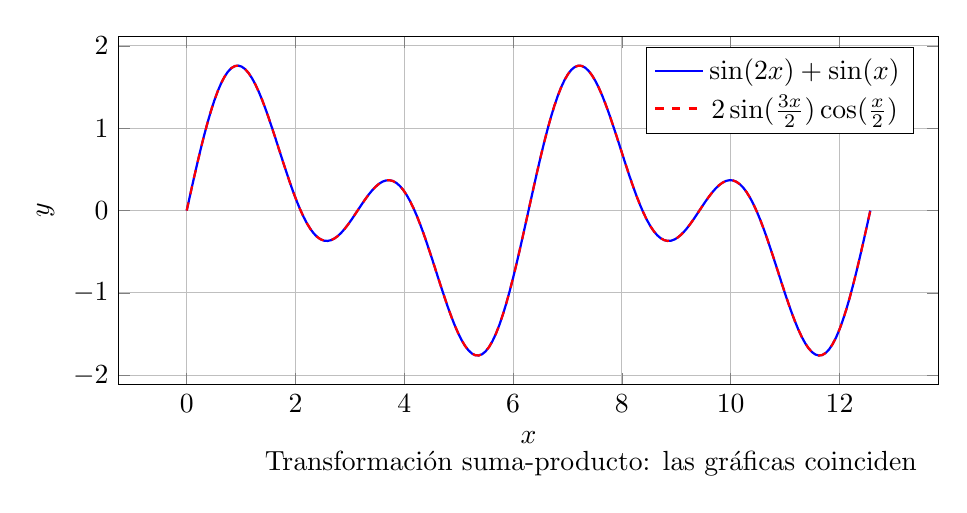
\begin{tikzpicture}[scale=1]
    % Gráfica ilustrativa de transformación suma-producto
    \begin{axis}[
        width=12cm,
        height=6cm,
        xlabel={$x$},
        ylabel={$y$},
        domain=0:4*pi,
        samples=200,
        grid=major,
        legend pos=north east,
        cycle list name=color list
    ]

    % Suma original
    \addplot[blue,thick] {sin(deg(2*x)) + sin(deg(x))};
    \addlegendentry{$\sin(2x) + \sin(x)$}

    % Producto equivalente
    \addplot[red,dashed,thick] {2*sin(deg(1.5*x))*cos(deg(0.5*x))};
    \addlegendentry{$2\sin(\frac{3x}{2})\cos(\frac{x}{2})$}

    \end{axis}

    \node at (6,-1) {Transformación suma-producto: las gráficas coinciden};
\end{tikzpicture}
\end{center}

\textbf{Observación importante:}
Las transformaciones suma-producto y producto-suma son muy útiles en:
\begin{itemize}
    \item Integración de funciones trigonométricas
    \item Análisis de ondas y señales
    \item Resolución de ecuaciones trigonométricas
    \item Simplificación de expresiones complejas
\end{itemize}

¡Fíjate cómo en la gráfica anterior, la suma de senos (línea azul) es idéntica al producto (línea roja punteada)! Esto demuestra que nuestras transformaciones son correctas.
\end{solucion}